% ============================================================================
% EC7205: Cloud Computing — Assignment 2 Report
% HealthSync: A Scalable Cloud-Native Healthcare Platform
% University of Ruhuna, Faculty of Engineering
% ============================================================================
\documentclass[12pt,a4paper]{article}

% ---- Core Packages ----
\usepackage[utf8]{inputenc}
\usepackage[T1]{fontenc}
\usepackage{textcomp}
\usepackage{amssymb}
\usepackage{graphicx}
\usepackage{titlesec}
\usepackage{setspace}
\usepackage{geometry}
\geometry{margin=0.82in}
\usepackage{listings}
\usepackage{xcolor}
\usepackage{float}
\usepackage{caption}
\usepackage{subcaption}
\usepackage{tikz}
\usepackage{booktabs}
\usepackage{tabularx}
\usepackage{enumitem}
\usepackage{fancybox}
\usepackage{mdframed}
\usepackage{multicol}

% ---- TikZ Libraries ----
\usetikzlibrary{shapes.geometric, arrows.meta, positioning, fit, backgrounds, calc, decorations.markings, patterns, shadows}

% ---- Azure Color Palette ----
\definecolor{azureBlue}{HTML}{0078D4}
\definecolor{azureDarkBlue}{HTML}{003366}
\definecolor{azureLightBlue}{HTML}{50E6FF}
\definecolor{azureGreen}{HTML}{7FBA00}
\definecolor{azureOrange}{HTML}{FF8C00}
\definecolor{azureRed}{HTML}{E81123}
\definecolor{azurePurple}{HTML}{8661C5}
\definecolor{azureYellow}{HTML}{FFB900}
\definecolor{azureTeal}{HTML}{00B294}
\definecolor{azurePink}{HTML}{E3008C}
\definecolor{azureGray}{HTML}{505050}
\definecolor{lightBg}{HTML}{F5F7FA}
\definecolor{cardBg}{HTML}{FFFFFF}
\definecolor{borderGray}{HTML}{D2D2D2}
\definecolor{softGreen}{HTML}{E8F5E9}
\definecolor{softBlue}{HTML}{E3F2FD}
\definecolor{softOrange}{HTML}{FFF3E0}
\definecolor{softPurple}{HTML}{F3E5F5}

% ---- Hyperlinks ----
\usepackage[colorlinks=true, linkcolor=azureDarkBlue, citecolor=black, urlcolor=azureBlue]{hyperref}

% ---- Code listing style ----
\lstset{
    basicstyle=\ttfamily\footnotesize,
    backgroundcolor=\color{gray!5},
    frame=single,
    rulecolor=\color{borderGray},
    breaklines=true,
    breakatwhitespace=true,
    numbers=none,
    tabsize=2,
    showstringspaces=false,
    keywordstyle=\bfseries\color{azureBlue},
    commentstyle=\itshape\color{azureGray},
    stringstyle=\color{azureTeal},
    captionpos=b
}

% ---- Formatting ----
\setstretch{1.15}
\titleformat{\section}{\large\bfseries\color{azureDarkBlue}}{\thesection.}{1em}{}
\titleformat{\subsection}{\normalsize\bfseries\color{azureBlue}}{\thesubsection.}{1em}{}
\titlespacing*{\section}{0pt}{12pt}{5pt}
\titlespacing*{\subsection}{0pt}{9pt}{4pt}

% ---- Page numbering ----
\pagestyle{plain}

% ---- Highlight box ----
\newmdenv[
  backgroundcolor=softBlue,
  linecolor=azureBlue,
  linewidth=1.5pt,
  roundcorner=4pt,
  innertopmargin=8pt,
  innerbottommargin=8pt,
  innerleftmargin=10pt,
  innerrightmargin=10pt
]{infobox}

% ============================================================================
%                            TITLE PAGE
% ============================================================================
\begin{document}

\begin{titlepage}
    \centering
    % University logo — place uor-logo.png in images/ folder
    % \includegraphics[width=3cm]{images/uor-logo.png}\par\vspace{0.8cm}
    
    \vspace*{1cm}
    {\LARGE \textbf{Department of Electrical and Information Engineering}}\\[0.4cm]
    {\Large \textbf{University of Ruhuna}}\\[0.3cm]
    {\large Faculty of Engineering}\\[1.5cm]
    
    {\Large \textbf{Assignment 02 --- Semester 7}}\\[0.2cm]
    {\large \textbf{Cloud Computing}}\\[0.2cm]
    {\large \textbf{EC7205}}\\[0.15cm]
    {\normalsize April 2026}\\[2cm]

    {\LARGE \textbf{HealthSync}}\\[0.3cm]
    {\large A Scalable, Secured, and Highly Available\\Cloud-Native Healthcare Platform}\\[2.5cm]

    % ---- Team details — EDIT THESE ----
    \begin{tabular}{@{}l l}
        \textbf{Group Members} & : EG/2021/4735 --- Piyumal Ranasinghe \\
                                & \phantom{: }EG/20XX/XXXX --- Member Two \\
                                & \phantom{: }EG/20XX/XXXX --- Member Three \\
                                & \phantom{: }EG/20XX/XXXX --- Member Four \\[0.3cm]
        \textbf{Date}          & : April 2026 \\
    \end{tabular}

    \vfill
\end{titlepage}

% ============================================================================
%                          1. INTRODUCTION
% ============================================================================
\section{Introduction}

\textbf{HealthSync} is a cloud-native healthcare platform connecting patients with doctors through an event-driven microservices architecture deployed entirely on \textbf{Microsoft Azure}. The system addresses real-world healthcare challenges: appointment booking, prescription management, secure patient records, real-time email notifications, and integrated Stripe payments.

\noindent The platform comprises \textbf{7 microservices} (6~Node.js + 1~Python), a \textbf{React~18 SPA} frontend, and \textbf{21 Azure resources}---all provisioned via \textbf{13 reusable Terraform modules} and deployed through \textbf{GitHub Actions} CI/CD pipelines.

\smallskip
\noindent\textbf{Technology Stack:}
\begin{multicols}{2}
\begin{itemize}[noitemsep,topsep=0pt]
    \item \textbf{Frontend:} React 18, Tailwind CSS, Vite
    \item \textbf{API Gateway:} Express.js, JWT, Helmet
    \item \textbf{Backend:} Node.js 20 / Python 3.11
    \item \textbf{Databases:} Cosmos DB, PostgreSQL 16, Redis 6
    \item \textbf{Messaging:} Azure Service Bus (3 queues)
    \item \textbf{Email:} Azure Communication Services
    \item \textbf{Compute:} Azure Container Apps
    \item \textbf{CDN:} Azure Front Door Standard
    \item \textbf{IaC:} Terraform $\geq$1.9 (azurerm \textasciitilde4.0)
    \item \textbf{CI/CD:} GitHub Actions (2 pipelines)
\end{itemize}
\end{multicols}

\noindent\textbf{Repositories:}
\begin{itemize}[noitemsep,topsep=2pt]
    \item Application: \url{https://github.com/PiyumalKK/HealthSync}
    \item Infrastructure (IaC): \url{https://github.com/PixelTech-Solutions/HealthSync-Infra}
    \item Terraform Reusable Template: \url{https://github.com/PixelTech-Solutions/Terraform}
\end{itemize}

% ============================================================================
%                          2. ARCHITECTURE
% ============================================================================
\section{Architecture}

Figure~\ref{fig:architecture} shows the complete architecture. Traffic enters through \textbf{Azure Front Door} (CDN + WAF), routing static requests (\texttt{/*}) to Blob Storage and API calls (\texttt{/api/*}) to the Gateway Container App. The gateway authenticates via JWT and proxies to six internal microservices. Async events flow through Service Bus queues to the always-on Notification Service.

% ---- Full-page architecture diagram (v3 — clean grid, no overlaps) ----
\begin{figure}[p]
\centering
\vspace*{-0.8cm}
\resizebox{0.97\textwidth}{!}{%
\begin{tikzpicture}[
    % — Styles —
    box/.style={rectangle, rounded corners=5pt, minimum height=2.8cm, text width=3.4cm,
                align=center, font=\footnotesize, drop shadow={opacity=0.12}},
    msvc/.style={rectangle, rounded corners=4pt, draw=azureBlue!50, fill=white,
                 text width=3.2cm, minimum height=2.4cm, align=center, font=\footnotesize},
    db/.style={cylinder, shape border rotate=90, aspect=0.3, minimum width=2.6cm,
               minimum height=2.4cm, font=\footnotesize, align=center},
    qbox/.style={rectangle, rounded corners=3pt, draw=azureOrange!60, fill=azureOrange!6,
                 text width=2.5cm, minimum height=1.1cm, align=center, font=\footnotesize},
    arr/.style={-{Stealth[length=2.5mm, width=1.8mm]}, semithick, color=azureGray!70},
    darr/.style={-{Stealth[length=2.5mm, width=1.8mm]}, dashed, semithick, color=azureOrange!70},
    secarr/.style={-{Stealth[length=2.5mm, width=1.8mm]}, densely dashed, semithick, color=azureGreen!60},
    lbl/.style={font=\tiny\itshape, color=azureGray, fill=white, inner sep=1pt},
]

% ==================== TITLE ====================
\node[font=\large\bfseries\color{azureDarkBlue}] at (2,3)
    {HealthSync Cloud Architecture --- 21 Azure Resources};

% ==================== ROW 0: USERS (y=0) ====================
\node[box, draw=azureGray, fill=white] (user) at (0,0)
    {
\includegraphics[height=1.4cm]{images/users.png}\\
     \textbf{Users}\\{\tiny Browser / Mobile}};

% ==================== ROW 1: FRONT DOOR (y=-4) ====================
\node[box, draw=azureBlue!70, fill=azureBlue!6, text width=3.2cm] (fd) at (0,-4)
    {
\includegraphics[height=1.4cm]{images/front-door-and-cdn-profiles.png}\\
     \textbf{Azure Front Door}\\{\tiny CDN + SSL + WAF}};

% User → FD: vertical
\draw[arr] (user.south) -- (fd.north);

% ==================== ROW 2: THREE ORIGINS + AUTH DB (y=-8.5) ====================
\node[box, draw=azureTeal!70, fill=azureTeal!6] (blob) at (-5,-8.5)
    {
\includegraphics[height=1.4cm]{images/storage-accounts-classic.png}\\
     \textbf{Blob Storage}\\{\tiny Static Website}\\{\tiny React SPA (\$web)}};

\node[box, draw=azureBlue!70, fill=azureBlue!6] (gw) at (0,-8.5)
    {
\includegraphics[height=1.4cm]{images/worker-container-app.png}\\
     \textbf{API Gateway}\\{\tiny Container App}\\{\tiny Port 8080 (EXT)}};

\node[box, draw=azurePurple!70, fill=azurePurple!6] (acr) at (5,-8.5)
    {
\includegraphics[height=1.4cm]{images/container-registries.png}\\
     \textbf{Container}\\{\tiny Registry (ACR)}\\{\tiny 7 Docker Images}};

\node[db, draw=azureTeal!70, fill=azureTeal!8] (authdb) at (10,-8.5)
    {
\includegraphics[height=1.1cm]{images/azure-cosmos-db.png}\\
     \textbf{Cosmos DB}\\{\tiny auth (users)}};

% FD → Blob: vertical down, horizontal left, vertical down (strict H/V)
\draw[arr] (fd.south) -- (0,-6.2) -- (-5,-6.2) -- (blob.north);
\node[lbl] at (-2.8,-6.2) {/* (static)};

% FD → GW: center, straight vertical
\draw[arr] (fd.south) -- (gw.north);
\node[lbl] at (0.8,-6.2) {/api/*};

% GW → Auth DB: vertical up, horizontal right, vertical down (strict H/V)
\draw[arr, azureTeal!50] (gw.north) -- (0,-6.5) -- (10,-6.5) -- (authdb.north);
\node[lbl] at (5.5,-6.2) {user lookup};

% ==================== CONTAINER APPS ENVIRONMENT (y=-11.5 to -21) ====================
\begin{scope}[on background layer]
    \draw[rounded corners=8pt, draw=azureBlue!40, dashed, line width=1pt, fill=softBlue!15]
         (-10.5,-11.5) rectangle (7,-21);
\end{scope}
\node[font=\tiny\bfseries\color{azureBlue}, anchor=north west] at (-10.3,-11.6)
    {Container Apps Environment --- Private Internal Network};

% ==================== ROW 3a: TOP 4 MICROSERVICES (y=-14) ====================
\node[msvc] (doc) at (-8,-14)
    {
\includegraphics[height=1.1cm]{images/worker-container-app.png}\\
     \textbf{Doctor}\\{\tiny Service --- 3002}};
\node[msvc] (appt) at (-4,-14)
    {
\includegraphics[height=1.1cm]{images/worker-container-app.png}\\
     \textbf{Appointment}\\{\tiny Service --- 3003}};
\node[msvc] (pat) at (0,-14)
    {
\includegraphics[height=1.1cm]{images/worker-container-app.png}\\
     \textbf{Patient}\\{\tiny Service --- 3001}};
\node[msvc] (presc) at (4,-14)
    {
\includegraphics[height=1.1cm]{images/worker-container-app.png}\\
     \textbf{Prescription}\\{\tiny Service --- 3004}};

% ==================== ROW 3b: BOTTOM 2 MICROSERVICES (y=-18.5) ====================
\node[msvc] (pay) at (-6,-18.5)
    {
\includegraphics[height=1.1cm]{images/worker-container-app.png}\\
     \textbf{Payment}\\{\tiny Service --- 3006}};
\node[msvc, draw=azureOrange!50, fill=azureOrange!4] (notif) at (2,-18.5)
    {
\includegraphics[height=1.1cm]{images/worker-container-app.png}\\
     \textbf{Notification}\\{\tiny Svc --- 3005 (always-on)}};

% ==================== GATEWAY → SERVICES (bus-bar routing, all H/V) ====================
% Vertical trunk from GW down to bus-bar at y=-12.5
\draw[semithick, azureBlue!50] (gw.south) -- (0,-12.5);
% Horizontal bus bar across top-4 services
\draw[semithick, azureBlue!50] (-8,-12.5) -- (4,-12.5);
% Vertical drops to each top service
\draw[arr, azureBlue!50] (-8,-12.5) -- (doc.north);
\draw[arr, azureBlue!50] (-4,-12.5) -- (appt.north);
\draw[arr, azureBlue!50] (0,-12.5) -- (pat.north);
\draw[arr, azureBlue!50] (4,-12.5) -- (presc.north);
% Second bus bar for bottom services at y=-16.8
\draw[semithick, azureBlue!50] (0,-12.5) -- (0,-16.8);
\draw[semithick, azureBlue!50] (-6,-16.8) -- (2,-16.8);
\draw[arr, azureBlue!50] (-6,-16.8) -- (pay.north);
\draw[arr, azureBlue!50] (2,-16.8) -- (notif.north);

% ==================== SERVICE BUS (right column, outside env box) ====================
\node[box, draw=azureOrange!70, fill=azureOrange!5, text width=2.5cm] (sb) at (12,-14)
    {
\includegraphics[height=1.4cm]{images/azure-service-bus.png}\\
     \textbf{Service Bus}\\{\tiny Async Messaging}};
\node[qbox] (q1) at (12,-17) {appointment\\-events};
\node[qbox] (q2) at (12,-19) {prescription\\-events};
\node[qbox] (q3) at (12,-20.5) {doctor-events};

% SB → queues: vertical
\draw[arr, azureOrange!60] (sb.south) -- (q1.north);
\draw[arr, azureOrange!60] (q1.south) -- (q2.north);
\draw[arr, azureOrange!60] (q2.south) -- (q3.north);

% Appt → q1: down, right, down, right (strict H/V)
\draw[darr] (appt.south) -- (-4,-15.8) -- (8,-15.8) -- (8,-17) -- (q1.west);
% Presc → q2: down, right, down, right (strict H/V)
\draw[darr] (presc.south) -- (4,-16.2) -- (9,-16.2) -- (9,-19) -- (q2.west);
% q1 → Notif: left, down, left (strict H/V)
\draw[darr] (q1.west) -- (8,-17) -- (8,-17.3) -- (notif.north east);
% q2 → Notif: left, up, left (strict H/V)
\draw[darr] (q2.west) -- (8,-19) -- (8,-18.5) -- (notif.east);

% ==================== ROW 4: DATABASES (y=-26) ====================
% PostgreSQL label and instances
\node[font=\footnotesize\bfseries\color{azureBlue}] at (-6.5,-23.5) {PostgreSQL 16};
\node[db, draw=azureBlue!70, fill=azureBlue!8] (pgdoc) at (-8,-26)
    {
\includegraphics[height=1.1cm]{images/azure-database-postgresql-server.png}\\
     \textbf{doctors}};
\node[db, draw=azureBlue!70, fill=azureBlue!8] (pgappt) at (-5,-26)
    {
\includegraphics[height=1.1cm]{images/azure-database-postgresql-server.png}\\
     \textbf{appointments}};
\node[db, draw=azureBlue!70, fill=azureBlue!8] (pgpay) at (-2,-26)
    {
\includegraphics[height=1.1cm]{images/azure-database-postgresql-server.png}\\
     \textbf{payments}};

% Cosmos DB label and instances
\node[font=\footnotesize\bfseries\color{azureTeal}] at (4,-23.5) {Cosmos DB (MongoDB API)};
\node[db, draw=azureTeal!70, fill=azureTeal!8] (cosmopat) at (1.5,-26)
    {
\includegraphics[height=1.1cm]{images/azure-cosmos-db.png}\\
     \textbf{patients}};
\node[db, draw=azureTeal!70, fill=azureTeal!8] (cosmopresc) at (4.5,-26)
    {
\includegraphics[height=1.1cm]{images/azure-cosmos-db.png}\\
     \textbf{prescriptions}};
\node[db, draw=azureTeal!70, fill=azureTeal!8] (cosmonot) at (7.5,-26)
    {
\includegraphics[height=1.1cm]{images/azure-cosmos-db.png}\\
     \textbf{notifications}};

% Redis (well below doctors DB)
\node[db, draw=azureRed!70, fill=azureRed!8] (redis) at (-8,-30)
    {
\includegraphics[height=1.1cm]{images/cache-redis.png}\\
     \textbf{Redis Cache}\\{\tiny 6380/TLS}};

% Service → DB arrows (all strict H/V via routing lane at y=-23)
\draw[arr, azureBlue!40] (doc.south) -- (-8,-23) -- (pgdoc.north);
\draw[arr, azureBlue!40] (appt.south) -- (-4,-23) -- (-5,-23) -- (pgappt.north);
\draw[arr, azureBlue!40] (pay.south) -- (-6,-23) -- (-2,-23) -- (pgpay.north);
\draw[arr, azureTeal!40] (pat.south) -- (0,-23) -- (1.5,-23) -- (cosmopat.north);
\draw[arr, azureTeal!40] (presc.south) -- (4,-23) -- (4.5,-23) -- (cosmopresc.north);
\draw[arr, azureTeal!40] (notif.south) -- (2,-23) -- (7.5,-23) -- (cosmonot.north);
% Doctor → Redis: down, left, down, right (strict H/V)
\draw[arr, azureRed!40] (doc.south) -- (-8,-23) -- (-10.5,-23) -- (-10.5,-30) -- (redis.west);

% ==================== ACR → pulls images (strict H/V around env box) ====================
\draw[arr, azurePurple!40, densely dashed] (acr.south) -- (5,-10.5) -- (7.3,-10.5) -- (7.3,-14) -- (presc.east);
\node[lbl] at (7.3,-12) {\rotatebox{90}{pulls images}};

% ==================== EXTERNAL SERVICES ====================
% Stripe (left side, below databases)
\node[box, draw=azureYellow!70, fill=azureYellow!5, text width=3cm] (stripe) at (-3,-30)
    {
\includegraphics[height=1.4cm]{images/stripe.png}\\
     \textbf{Stripe}\\{\tiny Payment Gateway}};

% ACS Email (right column, below queues)
\node[box, draw=azurePink!70, fill=azurePink!5, text width=3cm] (acs) at (12,-26)
    {
\includegraphics[height=1.4cm]{images/azure-communication-services.png}\\
     \textbf{ACS Email}\\{\tiny Communication Svc}\\{\tiny Sends notifications}};

% Pay → Stripe: down, horizontal, down (strict H/V)
\draw[arr, azureYellow!60] (pay.south) -- (-6,-23) -- (-3,-23) -- (stripe.north);
% Notif → ACS: down, horizontal, down (strict H/V)
\draw[arr, azurePink!60] (notif.south) -- (2,-23) -- (12,-23) -- (acs.north);

% ==================== SECURITY & OBSERVABILITY (right side panel — enlarged) ====================
\begin{scope}[on background layer]
    \draw[rounded corners=6pt, draw=azureGray!30, fill=softPurple!20, line width=0.8pt]
         (8.5,-28) rectangle (16,-36.5);
\end{scope}
\node[font=\normalsize\bfseries\color{azurePurple}, anchor=north west] at (9,-28.3)
    {Security \& Observability};

\node[box, draw=azurePurple!70, fill=azurePurple!5, text width=3cm] (logs) at (12.2,-30.5)
    {
\includegraphics[height=1.4cm]{images/log-analytics-workspaces.png}\\
     \textbf{Log Analytics}\\{\tiny Workspace}\\{\tiny All container logs}};

\node[box, draw=azureGreen!70, fill=azureGreen!5, text width=2.8cm] (kv) at (10.5,-34.5)
    {
\includegraphics[height=1.4cm]{images/key-vaults.png}\\
     \textbf{Key Vault}\\{\tiny 16 Secrets (RBAC)}};
\node[box, draw=azureOrange!70, fill=azureOrange!5, text width=2.8cm] (mi) at (14.5,-34.5)
    {
\includegraphics[height=1.4cm]{images/managed-identities.png}\\
     \textbf{Managed}\\{\tiny Identity}\\{\tiny Passwordless Auth}};

% MI → KV: horizontal
\draw[secarr] (mi.west) -- (kv.east);
\node[lbl] at (12.5,-33) {authenticates};

% ==================== LEGEND (y=-37.5) ====================
\node[anchor=north west, font=\footnotesize, text width=16cm] at (-10,-37.5) {
    \begin{tabular}{@{}cl@{\hspace{12pt}}cl@{\hspace{12pt}}cl@{}}
        \tikz\draw[arr, azureBlue!60] (0,0) -- (0.7,0); & Sync (HTTPS) &
        \tikz\draw[darr] (0,0) -- (0.7,0); & Async (Service Bus) &
        \tikz\draw[secarr] (0,0) -- (0.7,0); & Secrets / Identity \\[3pt]
        \tikz\fill[azureBlue!10, draw=azureBlue!70, rounded corners=2pt] (0,-0.08) rectangle (0.4,0.22); & PostgreSQL &
        \tikz\fill[azureTeal!10, draw=azureTeal!70, rounded corners=2pt] (0,-0.08) rectangle (0.4,0.22); & Cosmos DB &
        \tikz\fill[azureRed!10, draw=azureRed!70, rounded corners=2pt] (0,-0.08) rectangle (0.4,0.22); & Redis Cache \\
    \end{tabular}
};

\end{tikzpicture}
}
\caption{HealthSync complete cloud architecture --- 7 microservices, 21 Azure resources, fully provisioned via Terraform IaC.}
\label{fig:architecture}
\end{figure}

\subsection{Key Architecture Decisions}

\begin{table}[H]
\centering
\footnotesize
\caption{Architecture decisions mapped to cloud computing principles}
\begin{tabularx}{\textwidth}{@{}lXl@{}}
\toprule
\textbf{Decision} & \textbf{Rationale} & \textbf{Principle} \\
\midrule
7 Microservices & Independent scaling, deployment, fault isolation per domain & Scalability \\
API Gateway & Single entry for JWT auth, rate limiting, CORS, routing & Security \\
Database-per-service & Polyglot persistence (Cosmos + PG + Redis); no shared coupling & Loose coupling \\
Service Bus (3 queues) & Decouple producers from consumers; messages survive failures & Availability \\
Container Apps & Serverless auto-scale 0$\to$3; pay only for consumption & Elasticity \\
Key Vault + Managed ID & Zero secrets in code; passwordless Azure-to-Azure auth & Security \\
Terraform (13 modules) & Reproducible, version-controlled infrastructure & DevOps/IaC \\
\bottomrule
\end{tabularx}
\label{tab:decisions}
\end{table}

\subsection{Communication Methods}

\textbf{Synchronous (HTTPS):} Browser $\to$ Front Door $\to$ API Gateway $\to$ internal services for real-time request/response.

\noindent\textbf{Asynchronous (Service Bus):} Events published to queues (\texttt{appointment-events}, \texttt{prescription-events}, \texttt{doctor-events}); the Notification Service (\texttt{min\_replicas=1}) consumes and sends email via ACS. Booking returns in $<$200ms while notifications process asynchronously.

% ============================================================================
%                     3. IMPLEMENTATION STEPS
% ============================================================================
\section{Implementation Steps}

\subsection{Infrastructure as Code (Terraform)}

All 21 Azure resources are defined as \textbf{13 reusable Terraform modules} (resource-group, acr, container-app$\times$7, container-apps-env, managed-identity, storage-account, key-vault, front-door, communication-services, cosmos-db, postgresql, redis, service-bus) composed in a service layer. Infrastructure is \textbf{never provisioned manually}---all changes flow through CI/CD.

\noindent\textbf{Remote state:} Terraform state is stored in Azure Blob Storage (\texttt{stpixeltechstate/tfstate}) with state locking via Azure Blob leases, enabling safe team collaboration without state conflicts.

\noindent\textbf{Key Terraform features used:}
\begin{itemize}[noitemsep,topsep=2pt]
    \item \texttt{dynamic} blocks --- variable-length secret/env-var injection into Container Apps
    \item \texttt{lifecycle \{ ignore\_changes = [image] \}} --- prevents CI/CD image updates from causing Terraform drift
    \item \texttt{depends\_on} --- ensures correct resource ordering (e.g., Key Vault before Container Apps)
    \item \texttt{sensitive = true} --- masks secret values in plan output and logs
\end{itemize}

\subsection{CI/CD Pipelines}
\label{sec:infra-pipeline}

\textbf{Infrastructure pipeline} (\texttt{infra-dev.yml}) calls a reusable Terraform template (\href{https://github.com/PixelTech-Solutions/Terraform}{org-wide}) via \texttt{workflow\_call}. \texttt{TF\_VAR\_*} GitHub Secrets inject sensitive values. GitHub Environments provide manual approval gates.

\begin{figure}[H]
\centering
\resizebox{0.95\textwidth}{!}{%
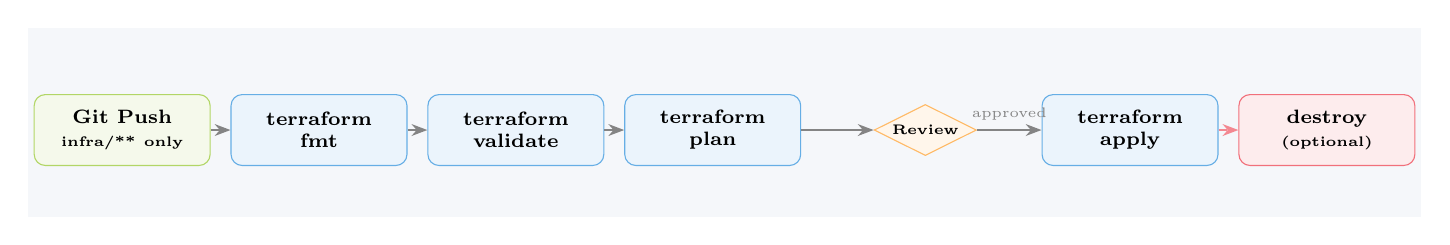
\begin{tikzpicture}[
    stage/.style={rectangle, rounded corners=4pt, draw=azureBlue!60, fill=azureBlue!8,
                  text width=2cm, minimum height=0.9cm, align=center, font=\scriptsize\bfseries},
    trigger/.style={rectangle, rounded corners=4pt, draw=azureGreen!60, fill=azureGreen!8,
                   text width=2cm, minimum height=0.9cm, align=center, font=\scriptsize\bfseries},
    gate/.style={diamond, draw=azureOrange!60, fill=azureOrange!8, 
                aspect=2, font=\scriptsize\bfseries, inner sep=1pt},
    arrow/.style={-{Stealth[length=2mm]}, thick, color=azureGray!70},
]
\fill[lightBg] (-1.2,-0.8) rectangle (16.5,1.6);
\node[trigger] (push) at (0,0.3) {Git Push\\{\tiny infra/** only}};
\node[stage] (fmt) at (2.5,0.3) {terraform\\fmt};
\node[stage] (val) at (5,0.3) {terraform\\validate};
\node[stage] (plan) at (7.5,0.3) {terraform\\plan};
\node[gate] (review) at (10.2,0.3) {\tiny Review};
\node[stage] (apply) at (12.8,0.3) {terraform\\apply};
\node[stage, draw=azureRed!60, fill=azureRed!8] (destroy) at (15.3,0.3) {destroy\\{\tiny (optional)}};
\draw[arrow] (push) -- (fmt);
\draw[arrow] (fmt) -- (val);
\draw[arrow] (val) -- (plan);
\draw[arrow] (plan) -- (review);
\draw[arrow] (review) -- node[above, font=\tiny] {approved} (apply);
\draw[arrow, dashed, azureRed!50] (apply) -- (destroy);
\end{tikzpicture}
}
\caption{Infrastructure pipeline (reusable template): format $\to$ validate $\to$ plan $\to$ manual approval $\to$ apply.}
\label{fig:infra-pipeline}
\end{figure}

\noindent\textbf{Application pipeline} (\texttt{deploy.yml}) uses manual dispatch with per-service selection. Docker images tagged with Git SHA for traceability and rollback.

\begin{figure}[H]
\centering
\resizebox{0.95\textwidth}{!}{%
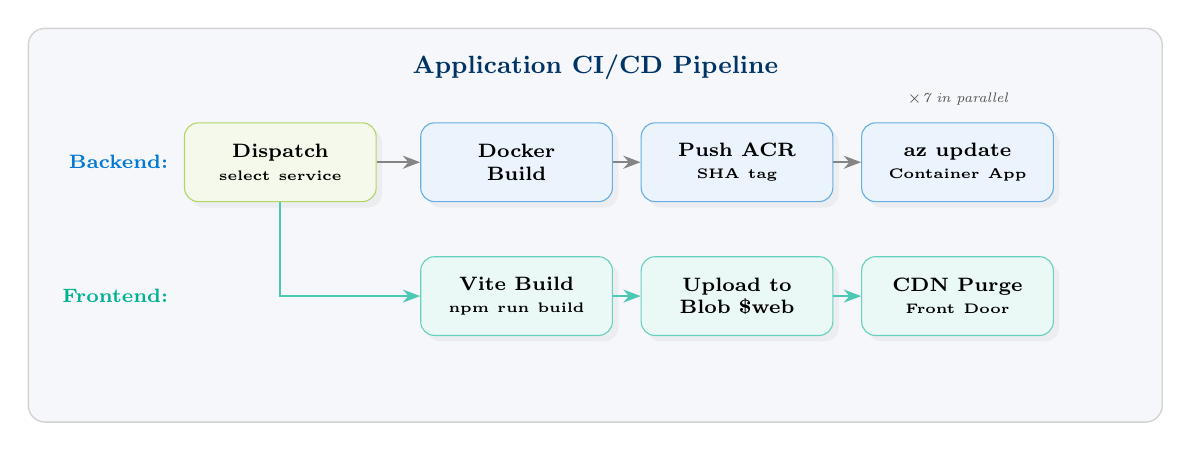
\begin{tikzpicture}[
    stage/.style={rectangle, rounded corners=5pt, draw=azureBlue!60, fill=azureBlue!8,
                  text width=2.2cm, minimum height=1cm, align=center, font=\scriptsize\bfseries,
                  drop shadow={opacity=0.08}},
    trigger/.style={rectangle, rounded corners=5pt, draw=azureGreen!60, fill=azureGreen!8,
                   text width=2.2cm, minimum height=1cm, align=center, font=\scriptsize\bfseries,
                   drop shadow={opacity=0.08}},
    arrow/.style={-{Stealth[length=2.2mm]}, thick, color=azureGray!70},
]
% Symmetric centered background
\fill[lightBg, rounded corners=6pt] (-3.2,-2.6) rectangle (11.2,2.4);
\draw[borderGray, rounded corners=6pt, line width=0.5pt] (-3.2,-2.6) rectangle (11.2,2.4);
\node[font=\small\bfseries\color{azureDarkBlue}] at (4,1.9) {Application CI/CD Pipeline};

% Backend row
\node[font=\scriptsize\bfseries\color{azureBlue}, anchor=east] at (-1.3, 0.7) {Backend:};
\node[trigger] (dispatch) at (0,0.7) {Dispatch\\{\tiny select service}};
\node[stage] (build) at (3,0.7) {Docker\\Build};
\node[stage] (push) at (5.8,0.7) {Push ACR\\{\tiny SHA tag}};
\node[stage] (deploy) at (8.6,0.7) {az update\\{\tiny Container App}};
\draw[arrow] (dispatch) -- (build);
\draw[arrow] (build) -- (push);
\draw[arrow] (push) -- (deploy);
\node[font=\tiny\itshape, color=azureGray, anchor=south] at (8.6,1.3) {$\times$7 in parallel};

% Frontend row
\node[font=\scriptsize\bfseries\color{azureTeal}, anchor=east] at (-1.3,-1) {Frontend:};
\node[stage, fill=azureTeal!8, draw=azureTeal!60] (fbuild) at (3,-1) {Vite Build\\{\tiny npm run build}};
\node[stage, fill=azureTeal!8, draw=azureTeal!60] (fupload) at (5.8,-1) {Upload to\\Blob \$web};
\node[stage, fill=azureTeal!8, draw=azureTeal!60] (fpurge) at (8.6,-1) {CDN Purge\\{\tiny Front Door}};
\draw[arrow, azureTeal!70] (dispatch) |- (fbuild);
\draw[arrow, azureTeal!70] (fbuild) -- (fupload);
\draw[arrow, azureTeal!70] (fupload) -- (fpurge);
\end{tikzpicture}
}
\caption{Application pipeline: per-service Docker build, ACR push, Container App update. Frontend uploads to Blob Storage.}
\label{fig:app-pipeline}
\end{figure}

\subsection{Security Implementation (Five Layers)}

\begin{enumerate}[noitemsep,topsep=2pt]
    \item \textbf{Network isolation:} Only API Gateway externally accessible; 6 services use private Container Apps DNS.
    \item \textbf{Authentication:} JWT access + httpOnly refresh tokens, signed with Key Vault secrets.
    \item \textbf{Authorization:} RBAC (patient, doctor, admin) enforced at gateway. Helmet.js headers (HSTS, CSP).
    \item \textbf{Secrets management:} 16 secrets in Key Vault (RBAC mode); Managed Identity reads at startup---zero passwords in code.
    \item \textbf{Transport encryption:} TLS everywhere: Front Door HTTPS, PG SSL, Redis 6380/TLS, Cosmos SSL, AMQPS. Rate limiting (50/15min auth, 500 API).
\end{enumerate}

\subsection{Scalability \& High Availability}

\begin{table}[H]
\centering
\footnotesize
\caption{Scalability mechanisms across the architecture}
\begin{tabularx}{\textwidth}{@{}l l X@{}}
\toprule
\textbf{Component} & \textbf{Mechanism} & \textbf{Details} \\
\midrule
Container Apps & Horizontal auto-scaling & 0$\to$3 replicas based on CPU/memory. Notification Service pinned at min=1. \\
Cosmos DB & Serverless (auto-RU) & Scales throughput automatically; no capacity planning needed. \\
PostgreSQL & Burstable B1ms & Can be upgraded to General Purpose or Memory Optimized via Terraform variable. \\
Front Door & Global CDN & 200+ edge locations, automatic origin failover via health probes. \\
Service Bus & Queue buffering & Messages persist if consumers are down; prevents data loss under load. \\
Redis & In-memory cache & Reduces PostgreSQL load by caching doctor listings (5-min TTL). \\
\bottomrule
\end{tabularx}
\end{table}

\noindent\textbf{High availability:} Cosmos DB provides built-in multi-region replication, PostgreSQL Flexible Server supports zone-redundant HA, Front Door health probes automatically failover between origins, and Container Apps restart failed replicas.

\subsection{Database Strategy}

A \textbf{polyglot persistence} approach matches database technology to data patterns:

\begin{itemize}[noitemsep]
    \item \textbf{Cosmos DB (MongoDB API, Serverless)} --- 4 databases: user accounts (\texttt{auth}), patient records, prescriptions, notifications. Flexible schema + serverless scaling.
    \item \textbf{PostgreSQL 16} --- 3 databases: doctor profiles with reviews, appointment bookings with time slots, payment transactions. ACID transactions + foreign key integrity.
    \item \textbf{Redis (Basic C0)} --- In-memory cache for Doctor Service. Reduces DB load for read-heavy doctor listing queries (5-min TTL).
\end{itemize}

\subsection{Extensibility}

Adding a new microservice (e.g., Lab Results) requires: (1) write service code with Dockerfile, (2) add a \texttt{module} block in \texttt{compute.tf} reusing the generic container-app module, (3) add a proxy route in the gateway, (4) run \texttt{terraform apply}, (5) deploy via existing CI/CD. No existing services need modification.

% ============================================================================
%                     4. CHALLENGES FACED
% ============================================================================
\section{Challenges Faced}

\begin{table}[H]
\centering
\footnotesize
\caption{Major challenges and their resolutions}
\begin{tabularx}{\textwidth}{@{}l X X@{}}
\toprule
\textbf{\#} & \textbf{Challenge} & \textbf{Resolution} \\
\midrule
1 & \textbf{CORS blocking.} Front Door FQDN not in allowed origins. & Added Front Door + Storage URLs to CORS whitelist; set \texttt{followRedirects: true}. \\
\addlinespace
2 & \textbf{Cosmos DB wire protocol errors.} Mongoose hit unsupported commands on serverless. & Pinned \texttt{server\_version = "4.2"} in Terraform; added \texttt{serverApi} compat. \\
\addlinespace
3 & \textbf{Redis TLS refused.} Defaulted to non-TLS port 6379. & Set \texttt{REDIS\_PORT=6380}, \texttt{REDIS\_TLS=true} in Container App env vars. \\
\addlinespace
4 & \textbf{SPA deep-link 404s.} Blob Storage returned 404 for \texttt{/about}. & Configured Front Door SPA rewrite rule: non-file URLs $\to$ \texttt{/index.html}. \\
\addlinespace
5 & \textbf{Email domain not linked to ACS.} Notification Service couldn't send emails. & Added \texttt{azurerm\_email\_communication\_service\_domain} association in Terraform. \\
\addlinespace
6 & \textbf{Internal proxy HTTPS loops.} Redirect loops between Container Apps. & Set \texttt{allow\_insecure = true} on ingress; \texttt{secure: false} on proxy middleware. \\
\bottomrule
\end{tabularx}
\end{table}

% ============================================================================
%                     5. LESSONS LEARNED
% ============================================================================
\section{Lessons Learned}

\begin{enumerate}[leftmargin=*]
    \item \textbf{IaC is essential for cloud-native development.} Terraform's modular approach let us destroy and recreate the entire 21-resource environment reliably. Manual Azure Portal configuration would be error-prone and non-reproducible.

    \item \textbf{Database-per-service enforces true microservice boundaries.} Separate databases eliminate hidden coupling---services communicate only through APIs or message queues, making independent scaling and redeployment straightforward.

    \item \textbf{Async messaging dramatically improves UX.} Appointment booking returns in $<$200ms because email notifications happen asynchronously via Service Bus, not inline with the API response.

    \item \textbf{Managed Identity eliminates secrets-in-code.} Passwordless Azure-to-Azure authentication via User-Assigned Managed Identity means no credentials in code or config files.

    \item \textbf{Cloud services have regional constraints.} Cosmos DB Serverless was unavailable in East US, requiring multi-region deployment (Cosmos in West US 2, PostgreSQL in North Europe)---unintentionally improving resilience.

    \item \textbf{Selective CI/CD matters for microservices.} Per-service deployment via workflow inputs prevents unnecessary rebuilds. Git SHA image tags enable instant rollback.

    \item \textbf{CDN + SPA requires explicit routing rules.} Without a catch-all rewrite rule at the Front Door level, single-page application deep links break with 404 errors---a cloud-specific challenge absent in local development.
\end{enumerate}

\end{document}
